\begin{frame}[fragile]{MPI Communication}
Host 15 MPI processes \\

\includegraphics[width=\textwidth]{mpih15}

Xeon Phi 15 MPI processes \\

\includegraphics[width=\textwidth]{mpi15}

Xeon Phi 30 MPI processes \\

\includegraphics[width=\textwidth]{mpi30}

Xeon Phi 60 MPI processes \\

\includegraphics[width=\textwidth]{mpi60}
\end{frame}
\begin{frame}[fragile]{Metrics}
\par{Hardware Metric}
\begin{tabular}{lc}
\hline
   CPU\_CLK\_UNHALTED: & 6106650000000\\  
   Instructions Retired: & 2563800000000\\
   CPI Rate:& 2.382\\
   L1 Misses:&  16030750000\\ 
   L1 Hit Ratio: & 0.984\\
    Estimated Latency Impact:& 203.415\\
\end{tabular}

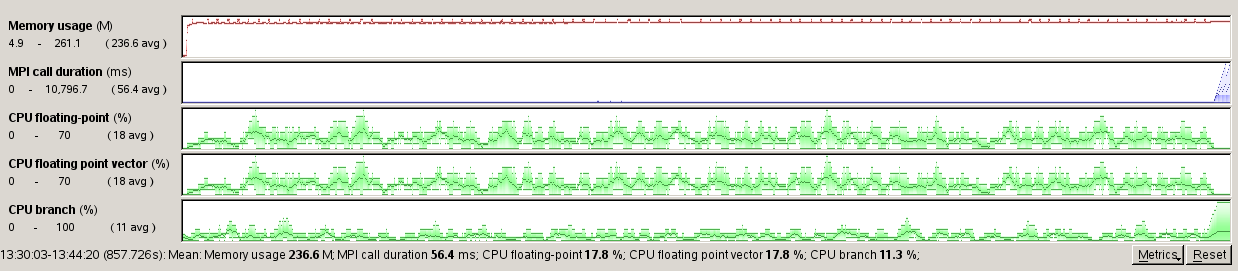
\includegraphics[width=\textwidth]{vec}

\end{frame}
\begin{frame}[fragile]{Logical CPU balance}
\vspace{20mm}
\begin{figure}
\begin{tikzpicture}[font=\footnotesize,xshift=-25mm,yshift=-17mm]
\begin{axis}[
scale only axis,
xmin=  1,xmax=240,
minor tick num =4,
every tick/.style={thick},
xlabel=hw threads, ylabel=time/s,
width=0.55\textwidth,
]
\addplot +[blue,thick] table[x index=0, y index=  1] {figures/vtune.dat};
\end{axis}
\end{tikzpicture}
\end{figure}
\vspace{20mm}
\par{15 MPI processes each 4 threads running on Xeon Phi}
\end{frame}
\begin{frame}[shrink,fragile]{Vectorisation}
some challenging pattern
\begin{fortrancode*}{}
  Do iz=nlz0e+1,nlz1s-1
     iz1=iz-nlz0e
     iz2=iz-nlz1s
     Do iy=nly0e+1,nly1s-1
        iy1=iy-nly0e
        iy2=iy-nly1s
        Do ix=nlx0e+1,nlx1s-1
           ix1=ix-nlx0e
           ix2=ix-nlx1s
           Do ipass=1,2
              If ( (ipass == 1) .or.                  &
                   (ix1 >=  1 .and. ix1 <=  nlp) .or. &
                   (ix2 <= -1 .and. ix2 >= -nlp) .or. &
                   (iy1 >=  1 .and. iy1 <=  nlp) .or. &
                   (iy2 <= -1 .and. iy2 >= -nlp) .or. &
                   (iz1 >=  1 .and. iz1 <=  nlp) .or. &
                   (iz2 <= -1 .and. iz2 >= -nlp) ) Then
                 ic=1+ix+(nlx+2*nlp)*(iy+(nly+2*nlp)*iz)
                 Do ii=lct_start(ic),lct_start(ic+1)-1
                    i=at_list(ii) 
                     Do kk=ipass,nsbcll
                       If (ipass ==  1) 
                          jx=ix+nix(kk)
                          jy=iy+niy(kk)
                          jz=iz+niz(kk)
                       Else 
                          jx=ix-nix(kk)
                          jy=iy-niy(kk)
                          jz=iz-niz(kk)
                       End If
                       If ( (ipass == 1 ) .or.                    &
                            (jx <= nlx0e) .or. (jx >= nlx1s) .or. &
                            (jy <= nly0e) .or. (jy >= nly1s) .or. &
                            (jz <= nlz0e) .or. (jz >= nlz1s) ) Then
                            jc=1+jx+(nlx+2*nlp)*(jy+(nly+2*nlp)*jz)

\end{fortrancode*}
% \begin{fortrancode*}{}
%  Do iz=nlz0e+1,nlz1s-1
%      iz1=iz-nlz0e
%      iz2=iz-nlz1s
%      Do iy=nly0e+1,nly1s-1
%         iy1=iy-nly0e
%         iy2=iy-nly1s
%         Do ix=nlx0e+1,nlx1s-1
%            ix1=ix-nlx0e
%            ix2=ix-nlx1s
%            Do ipass=1,2
% 
% \end{fortrancode*}
\end{frame}

